\documentclass[]{article}
\usepackage{lmodern}
\usepackage{amssymb,amsmath}
\usepackage{ifxetex,ifluatex}
\usepackage{fixltx2e} % provides \textsubscript
\ifnum 0\ifxetex 1\fi\ifluatex 1\fi=0 % if pdftex
  \usepackage[T1]{fontenc}
  \usepackage[utf8]{inputenc}
\else % if luatex or xelatex
  \ifxetex
    \usepackage{mathspec}
  \else
    \usepackage{fontspec}
  \fi
  \defaultfontfeatures{Ligatures=TeX,Scale=MatchLowercase}
\fi
% use upquote if available, for straight quotes in verbatim environments
\IfFileExists{upquote.sty}{\usepackage{upquote}}{}
% use microtype if available
\IfFileExists{microtype.sty}{%
\usepackage{microtype}
\UseMicrotypeSet[protrusion]{basicmath} % disable protrusion for tt fonts
}{}
\usepackage[margin=1in]{geometry}
\usepackage{hyperref}
\hypersetup{unicode=true,
            pdftitle={Cwong Final Project},
            pdfauthor={Calvin Wong},
            pdfborder={0 0 0},
            breaklinks=true}
\urlstyle{same}  % don't use monospace font for urls
\usepackage{color}
\usepackage{fancyvrb}
\newcommand{\VerbBar}{|}
\newcommand{\VERB}{\Verb[commandchars=\\\{\}]}
\DefineVerbatimEnvironment{Highlighting}{Verbatim}{commandchars=\\\{\}}
% Add ',fontsize=\small' for more characters per line
\usepackage{framed}
\definecolor{shadecolor}{RGB}{248,248,248}
\newenvironment{Shaded}{\begin{snugshade}}{\end{snugshade}}
\newcommand{\KeywordTok}[1]{\textcolor[rgb]{0.13,0.29,0.53}{\textbf{#1}}}
\newcommand{\DataTypeTok}[1]{\textcolor[rgb]{0.13,0.29,0.53}{#1}}
\newcommand{\DecValTok}[1]{\textcolor[rgb]{0.00,0.00,0.81}{#1}}
\newcommand{\BaseNTok}[1]{\textcolor[rgb]{0.00,0.00,0.81}{#1}}
\newcommand{\FloatTok}[1]{\textcolor[rgb]{0.00,0.00,0.81}{#1}}
\newcommand{\ConstantTok}[1]{\textcolor[rgb]{0.00,0.00,0.00}{#1}}
\newcommand{\CharTok}[1]{\textcolor[rgb]{0.31,0.60,0.02}{#1}}
\newcommand{\SpecialCharTok}[1]{\textcolor[rgb]{0.00,0.00,0.00}{#1}}
\newcommand{\StringTok}[1]{\textcolor[rgb]{0.31,0.60,0.02}{#1}}
\newcommand{\VerbatimStringTok}[1]{\textcolor[rgb]{0.31,0.60,0.02}{#1}}
\newcommand{\SpecialStringTok}[1]{\textcolor[rgb]{0.31,0.60,0.02}{#1}}
\newcommand{\ImportTok}[1]{#1}
\newcommand{\CommentTok}[1]{\textcolor[rgb]{0.56,0.35,0.01}{\textit{#1}}}
\newcommand{\DocumentationTok}[1]{\textcolor[rgb]{0.56,0.35,0.01}{\textbf{\textit{#1}}}}
\newcommand{\AnnotationTok}[1]{\textcolor[rgb]{0.56,0.35,0.01}{\textbf{\textit{#1}}}}
\newcommand{\CommentVarTok}[1]{\textcolor[rgb]{0.56,0.35,0.01}{\textbf{\textit{#1}}}}
\newcommand{\OtherTok}[1]{\textcolor[rgb]{0.56,0.35,0.01}{#1}}
\newcommand{\FunctionTok}[1]{\textcolor[rgb]{0.00,0.00,0.00}{#1}}
\newcommand{\VariableTok}[1]{\textcolor[rgb]{0.00,0.00,0.00}{#1}}
\newcommand{\ControlFlowTok}[1]{\textcolor[rgb]{0.13,0.29,0.53}{\textbf{#1}}}
\newcommand{\OperatorTok}[1]{\textcolor[rgb]{0.81,0.36,0.00}{\textbf{#1}}}
\newcommand{\BuiltInTok}[1]{#1}
\newcommand{\ExtensionTok}[1]{#1}
\newcommand{\PreprocessorTok}[1]{\textcolor[rgb]{0.56,0.35,0.01}{\textit{#1}}}
\newcommand{\AttributeTok}[1]{\textcolor[rgb]{0.77,0.63,0.00}{#1}}
\newcommand{\RegionMarkerTok}[1]{#1}
\newcommand{\InformationTok}[1]{\textcolor[rgb]{0.56,0.35,0.01}{\textbf{\textit{#1}}}}
\newcommand{\WarningTok}[1]{\textcolor[rgb]{0.56,0.35,0.01}{\textbf{\textit{#1}}}}
\newcommand{\AlertTok}[1]{\textcolor[rgb]{0.94,0.16,0.16}{#1}}
\newcommand{\ErrorTok}[1]{\textcolor[rgb]{0.64,0.00,0.00}{\textbf{#1}}}
\newcommand{\NormalTok}[1]{#1}
\usepackage{longtable,booktabs}
\usepackage{graphicx,grffile}
\makeatletter
\def\maxwidth{\ifdim\Gin@nat@width>\linewidth\linewidth\else\Gin@nat@width\fi}
\def\maxheight{\ifdim\Gin@nat@height>\textheight\textheight\else\Gin@nat@height\fi}
\makeatother
% Scale images if necessary, so that they will not overflow the page
% margins by default, and it is still possible to overwrite the defaults
% using explicit options in \includegraphics[width, height, ...]{}
\setkeys{Gin}{width=\maxwidth,height=\maxheight,keepaspectratio}
\IfFileExists{parskip.sty}{%
\usepackage{parskip}
}{% else
\setlength{\parindent}{0pt}
\setlength{\parskip}{6pt plus 2pt minus 1pt}
}
\setlength{\emergencystretch}{3em}  % prevent overfull lines
\providecommand{\tightlist}{%
  \setlength{\itemsep}{0pt}\setlength{\parskip}{0pt}}
\setcounter{secnumdepth}{0}
% Redefines (sub)paragraphs to behave more like sections
\ifx\paragraph\undefined\else
\let\oldparagraph\paragraph
\renewcommand{\paragraph}[1]{\oldparagraph{#1}\mbox{}}
\fi
\ifx\subparagraph\undefined\else
\let\oldsubparagraph\subparagraph
\renewcommand{\subparagraph}[1]{\oldsubparagraph{#1}\mbox{}}
\fi

%%% Use protect on footnotes to avoid problems with footnotes in titles
\let\rmarkdownfootnote\footnote%
\def\footnote{\protect\rmarkdownfootnote}

%%% Change title format to be more compact
\usepackage{titling}

% Create subtitle command for use in maketitle
\providecommand{\subtitle}[1]{
  \posttitle{
    \begin{center}\large#1\end{center}
    }
}

\setlength{\droptitle}{-2em}

  \title{Cwong Final Project}
    \pretitle{\vspace{\droptitle}\centering\huge}
  \posttitle{\par}
    \author{Calvin Wong}
    \preauthor{\centering\large\emph}
  \postauthor{\par}
      \predate{\centering\large\emph}
  \postdate{\par}
    \date{5/20/2019}


\begin{document}
\maketitle

Computational Mathematics

\section{+ setup, error=TRUE}\label{setup-errortrue}

\begin{Shaded}
\begin{Highlighting}[]
\KeywordTok{library}\NormalTok{(readr)}
\KeywordTok{library}\NormalTok{(tidyverse)}
\end{Highlighting}
\end{Shaded}

\begin{verbatim}
## -- Attaching packages ---------------------------------------------------------------------------------- tidyverse 1.2.1 --
\end{verbatim}

\begin{verbatim}
## v ggplot2 3.1.1     v purrr   0.3.2
## v tibble  2.1.1     v dplyr   0.8.1
## v tidyr   0.8.3     v stringr 1.4.0
## v ggplot2 3.1.1     v forcats 0.4.0
\end{verbatim}

\begin{verbatim}
## Warning: package 'ggplot2' was built under R version 3.5.2
\end{verbatim}

\begin{verbatim}
## Warning: package 'tibble' was built under R version 3.5.2
\end{verbatim}

\begin{verbatim}
## Warning: package 'tidyr' was built under R version 3.5.2
\end{verbatim}

\begin{verbatim}
## Warning: package 'purrr' was built under R version 3.5.2
\end{verbatim}

\begin{verbatim}
## Warning: package 'dplyr' was built under R version 3.5.2
\end{verbatim}

\begin{verbatim}
## Warning: package 'stringr' was built under R version 3.5.2
\end{verbatim}

\begin{verbatim}
## Warning: package 'forcats' was built under R version 3.5.2
\end{verbatim}

\begin{verbatim}
## -- Conflicts ------------------------------------------------------------------------------------- tidyverse_conflicts() --
## x dplyr::filter() masks stats::filter()
## x dplyr::lag()    masks stats::lag()
\end{verbatim}

\begin{Shaded}
\begin{Highlighting}[]
\KeywordTok{library}\NormalTok{(corrplot)}
\end{Highlighting}
\end{Shaded}

\begin{verbatim}
## corrplot 0.84 loaded
\end{verbatim}

\begin{Shaded}
\begin{Highlighting}[]
\KeywordTok{library}\NormalTok{(pracma)}
\end{Highlighting}
\end{Shaded}

\begin{verbatim}
## Warning: package 'pracma' was built under R version 3.5.2
\end{verbatim}

\begin{verbatim}
## 
## Attaching package: 'pracma'
\end{verbatim}

\begin{verbatim}
## The following object is masked from 'package:purrr':
## 
##     cross
\end{verbatim}

\begin{Shaded}
\begin{Highlighting}[]
\KeywordTok{library}\NormalTok{(MASS)}
\end{Highlighting}
\end{Shaded}

\begin{verbatim}
## Warning: package 'MASS' was built under R version 3.5.2
\end{verbatim}

\begin{verbatim}
## 
## Attaching package: 'MASS'
\end{verbatim}

\begin{verbatim}
## The following object is masked from 'package:dplyr':
## 
##     select
\end{verbatim}

\begin{Shaded}
\begin{Highlighting}[]
\KeywordTok{library}\NormalTok{(gmodels)}
\KeywordTok{library}\NormalTok{(tinytex)}
\end{Highlighting}
\end{Shaded}

\begin{verbatim}
## Warning: package 'tinytex' was built under R version 3.5.2
\end{verbatim}

Your final is due by the end of the last week of class. You should post
your solutions to your GitHub account or RPubs. You are also expected to
make a short presentation via YouTube and post that recording to the
board. This project will show off your ability to understand the
elements of the class.

\section{Problem 1.}\label{problem-1.}

Using R, generate a random variable X that has 10,000 random uniform
numbers from 1 to N, where N can be any number of your choosing greater
than or equal to 6. Then generate a random variable Y that has 10,000
random normal numbers with a mean of u = O = (N+1)/2.

\begin{Shaded}
\begin{Highlighting}[]
\NormalTok{N =}\StringTok{ }\DecValTok{100}
\NormalTok{X <-}\StringTok{ }\KeywordTok{runif}\NormalTok{(}\DecValTok{10000}\NormalTok{, }\DataTypeTok{min =} \DecValTok{1}\NormalTok{, }\DataTypeTok{max =} \DecValTok{100}\NormalTok{)}
\NormalTok{Y <-}\StringTok{ }\KeywordTok{rnorm}\NormalTok{(}\DecValTok{10000}\NormalTok{, }\DataTypeTok{mean =}\NormalTok{ (N}\OperatorTok{+}\DecValTok{1}\NormalTok{)}\OperatorTok{/}\DecValTok{2}\NormalTok{)}
\end{Highlighting}
\end{Shaded}

Probability. Calculate as a minimum the below probabilities a through c.
Assume the small letter ``x'' is estimated as the median of the X
variable, and the small letter ``y'' is estimated as the 1st quartile of
the Y variable. Interpret the meaning of all probabilities.

\subsection{5 points}\label{points}

\begin{enumerate}
\def\labelenumi{\alph{enumi}.}
\tightlist
\item
  P(X\textgreater{}x \textbar{} X\textgreater{}y)
\end{enumerate}

P(X\textgreater{}x \textbar{} Y\textgreater{}y) = P(X\textgreater{}x and
Y\textgreater{}y) / P(Y\textgreater{}y)

\begin{Shaded}
\begin{Highlighting}[]
\NormalTok{x <-}\StringTok{ }\KeywordTok{median}\NormalTok{(X)}
\NormalTok{y <-}\StringTok{ }\KeywordTok{quantile}\NormalTok{(Y, .}\DecValTok{25}\NormalTok{)}

\KeywordTok{sum}\NormalTok{(X}\OperatorTok{>}\NormalTok{x }\OperatorTok{&}\StringTok{ }\NormalTok{X}\OperatorTok{>}\NormalTok{y)}\OperatorTok{/}\KeywordTok{sum}\NormalTok{(X}\OperatorTok{>}\NormalTok{y)}
\end{Highlighting}
\end{Shaded}

\begin{verbatim}
## [1] 1
\end{verbatim}

\subsection{b. P(X\textgreater{}x, Y\textgreater{}y)}\label{b.-pxx-yy}

P(X\textgreater{}x, Y\textgreater{}y) = P(X\textgreater{}x) *
P(Y\textgreater{}y)

\begin{Shaded}
\begin{Highlighting}[]
\KeywordTok{sum}\NormalTok{(X}\OperatorTok{>}\NormalTok{x }\OperatorTok{&}\StringTok{ }\NormalTok{Y}\OperatorTok{>}\NormalTok{y)}\OperatorTok{/}\KeywordTok{length}\NormalTok{(X)}
\end{Highlighting}
\end{Shaded}

\begin{verbatim}
## [1] 0.3742
\end{verbatim}

\subsection{c. P(Xy)}\label{c.-pxy}

P(Xy) = P(Xy) / P(X\textgreater{}y)

\begin{Shaded}
\begin{Highlighting}[]
\KeywordTok{sum}\NormalTok{(X}\OperatorTok{<}\NormalTok{x }\OperatorTok{&}\StringTok{ }\NormalTok{X}\OperatorTok{>}\NormalTok{y)}\OperatorTok{/}\KeywordTok{sum}\NormalTok{(X}\OperatorTok{>}\NormalTok{y)}
\end{Highlighting}
\end{Shaded}

\begin{verbatim}
## [1] 0
\end{verbatim}

\subsection{5 points. Investigate whether P(X\textgreater{}x and
Y\textgreater{}y)=P(X\textgreater{}x)P(Y\textgreater{}y) by building a
table and evaluating the marginal and joint
probabilities.}\label{points.-investigate-whether-pxx-and-yypxxpyy-by-building-a-table-and-evaluating-the-marginal-and-joint-probabilities.}

\begin{Shaded}
\begin{Highlighting}[]
\NormalTok{tab <-}\StringTok{ }\KeywordTok{c}\NormalTok{(}\KeywordTok{sum}\NormalTok{(X }\OperatorTok{<}\StringTok{ }\NormalTok{x }\OperatorTok{&}\StringTok{ }\NormalTok{Y }\OperatorTok{<}\StringTok{ }\NormalTok{y), }\KeywordTok{sum}\NormalTok{(X }\OperatorTok{<}\StringTok{ }\NormalTok{x }\OperatorTok{&}\StringTok{ }\NormalTok{Y }\OperatorTok{>}\StringTok{ }\NormalTok{y))}
\NormalTok{tab <-}\StringTok{ }\KeywordTok{rbind}\NormalTok{(tab, }\KeywordTok{c}\NormalTok{(}\KeywordTok{sum}\NormalTok{(X}\OperatorTok{>}\NormalTok{x }\OperatorTok{&}\StringTok{ }\NormalTok{Y }\OperatorTok{<}\StringTok{ }\NormalTok{y), }\KeywordTok{sum}\NormalTok{(X }\OperatorTok{>}\StringTok{ }\NormalTok{x }\OperatorTok{&}\StringTok{ }\NormalTok{Y }\OperatorTok{>}\StringTok{ }\NormalTok{y)))}
\NormalTok{tab <-}\StringTok{ }\KeywordTok{cbind}\NormalTok{(tab, tab[,}\DecValTok{1}\NormalTok{] }\OperatorTok{+}\StringTok{ }\NormalTok{tab[,}\DecValTok{2}\NormalTok{])}
\NormalTok{tab <-}\StringTok{ }\KeywordTok{rbind}\NormalTok{(tab, tab[}\DecValTok{1}\NormalTok{,] }\OperatorTok{+}\StringTok{ }\NormalTok{tab[}\DecValTok{2}\NormalTok{,])}
\KeywordTok{colnames}\NormalTok{(tab) <-}\StringTok{ }\KeywordTok{c}\NormalTok{(}\StringTok{"Y<y"}\NormalTok{, }\StringTok{"Y>y"}\NormalTok{, }\StringTok{"Total"}\NormalTok{)}
\KeywordTok{rownames}\NormalTok{(tab) <-}\StringTok{ }\KeywordTok{c}\NormalTok{(}\StringTok{"X<x"}\NormalTok{, }\StringTok{"X>x"}\NormalTok{, }\StringTok{"Total"}\NormalTok{)}
\NormalTok{knitr}\OperatorTok{::}\KeywordTok{kable}\NormalTok{(tab)}
\end{Highlighting}
\end{Shaded}

\begin{longtable}[]{@{}lrrr@{}}
\toprule
& Y\textless{}y & Y\textgreater{}y & Total\tabularnewline
\midrule
\endhead
X\textless{}x & 1242 & 3758 & 5000\tabularnewline
X\textgreater{}x & 1258 & 3742 & 5000\tabularnewline
Total & 2500 & 7500 & 10000\tabularnewline
\bottomrule
\end{longtable}

\subsection{5 points. Check to see if independence holds by using
Fisher's Exact Test and the Chi Square Test. What is the difference
between the two? Which is most
appropriate?}\label{points.-check-to-see-if-independence-holds-by-using-fishers-exact-test-and-the-chi-square-test.-what-is-the-difference-between-the-two-which-is-most-appropriate}

\begin{Shaded}
\begin{Highlighting}[]
\KeywordTok{fisher.test}\NormalTok{(}\KeywordTok{table}\NormalTok{(X}\OperatorTok{>}\NormalTok{x,Y}\OperatorTok{>}\NormalTok{y))}
\end{Highlighting}
\end{Shaded}

\begin{verbatim}
## 
##  Fisher's Exact Test for Count Data
## 
## data:  table(X > x, Y > y)
## p-value = 0.729
## alternative hypothesis: true odds ratio is not equal to 1
## 95 percent confidence interval:
##  0.8970473 1.0773733
## sample estimates:
## odds ratio 
##  0.9830765
\end{verbatim}

\begin{Shaded}
\begin{Highlighting}[]
\KeywordTok{chisq.test}\NormalTok{(}\KeywordTok{table}\NormalTok{(X}\OperatorTok{>}\NormalTok{x,Y}\OperatorTok{>}\NormalTok{y))}
\end{Highlighting}
\end{Shaded}

\begin{verbatim}
## 
##  Pearson's Chi-squared test with Yates' continuity correction
## 
## data:  table(X > x, Y > y)
## X-squared = 0.12, df = 1, p-value = 0.729
\end{verbatim}

\section{Problem 2}\label{problem-2}

You are to register for Kaggle.com (free) and compete in the House
Prices: Advanced Regression Techniques competition.
\url{https://www.kaggle.com/c/house-prices-advanced-regression-techniques}
. I want you to do the following.

\begin{Shaded}
\begin{Highlighting}[]
\NormalTok{test <-}\StringTok{ }\KeywordTok{read.csv}\NormalTok{(}\StringTok{'https://raw.githubusercontent.com/cwong79/DATA605/master/test.csv'}\NormalTok{)}
\NormalTok{train <-}\StringTok{ }\KeywordTok{read.csv}\NormalTok{(}\StringTok{'https://raw.githubusercontent.com/cwong79/DATA605/master/train.csv'}\NormalTok{)}
\end{Highlighting}
\end{Shaded}

\subsection{5 points. Descriptive and Inferential Statistics. Provide
univariate descriptive statistics and appropriate plots for the training
data set. Provide a scatterplot matrix for at least two of the
independent variables and the dependent variable. Derive a correlation
matrix for any three quantitative variables in the dataset. Test the
hypotheses that the correlations between each pairwise set of variables
is 0 and provide an 80\% confidence interval. Discuss the meaning of
your analysis. Would you be worried about familywise error? Why or why
not?}\label{points.-descriptive-and-inferential-statistics.-provide-univariate-descriptive-statistics-and-appropriate-plots-for-the-training-data-set.-provide-a-scatterplot-matrix-for-at-least-two-of-the-independent-variables-and-the-dependent-variable.-derive-a-correlation-matrix-for-any-three-quantitative-variables-in-the-dataset.-test-the-hypotheses-that-the-correlations-between-each-pairwise-set-of-variables-is-0-and-provide-an-80-confidence-interval.-discuss-the-meaning-of-your-analysis.-would-you-be-worried-about-familywise-error-why-or-why-not}

\begin{Shaded}
\begin{Highlighting}[]
\NormalTok{train.df <-}\StringTok{ }\KeywordTok{data.frame}\NormalTok{(train)}
\NormalTok{trainsub <-}\StringTok{ }\NormalTok{train.df[, }\KeywordTok{c}\NormalTok{(}\DecValTok{1}\NormalTok{, }\DecValTok{2}\NormalTok{, }\DecValTok{5}\NormalTok{, }\DecValTok{20}\NormalTok{, }\DecValTok{35}\NormalTok{, }\DecValTok{44}\NormalTok{, }\DecValTok{45}\NormalTok{, }\DecValTok{47}\NormalTok{, }\DecValTok{55}\NormalTok{, }\DecValTok{78}\NormalTok{, }\DecValTok{81}\NormalTok{)]}
\NormalTok{t <-}\KeywordTok{cor}\NormalTok{(trainsub)}
\KeywordTok{corrplot}\NormalTok{(t, }\DataTypeTok{method=}\StringTok{"circle"}\NormalTok{)}
\end{Highlighting}
\end{Shaded}

\includegraphics{Cwong_Final_Project_files/figure-latex/unnamed-chunk-9-1.pdf}

Base on the correlation graph above, I will choose LotArea and GrLivArea
as my independent variables and SalePrice as my dependent.

\begin{Shaded}
\begin{Highlighting}[]
\NormalTok{trainsub1 <-}\StringTok{ }\NormalTok{train.df[, }\KeywordTok{c}\NormalTok{(}\DecValTok{5}\NormalTok{, }\DecValTok{47}\NormalTok{, }\DecValTok{81}\NormalTok{)]}
\end{Highlighting}
\end{Shaded}

\subsubsection{LotArea}\label{lotarea}

Null Hypothesis: The correlation between LotArea and SalePrice is 0
Alternative Hypothesis: The correlation between LotArea and SalePrice is
other than 0

\begin{Shaded}
\begin{Highlighting}[]
\NormalTok{lm1 <-}\StringTok{ }\KeywordTok{lm}\NormalTok{(trainsub1}\OperatorTok{$}\NormalTok{LotArea }\OperatorTok{~}\StringTok{ }\NormalTok{trainsub1}\OperatorTok{$}\NormalTok{SalePrice)}
\KeywordTok{summary}\NormalTok{(lm1)}
\end{Highlighting}
\end{Shaded}

\begin{verbatim}
## 
## Call:
## lm(formula = trainsub1$LotArea ~ trainsub1$SalePrice)
## 
## Residuals:
##    Min     1Q Median     3Q    Max 
## -13593  -2751   -914   1140 198295 
## 
## Coefficients:
##                      Estimate Std. Error t value Pr(>|t|)    
## (Intercept)         4.519e+03  6.271e+02   7.207 9.16e-13 ***
## trainsub1$SalePrice 3.315e-02  3.174e-03  10.445  < 2e-16 ***
## ---
## Signif. codes:  0 '***' 0.001 '**' 0.01 '*' 0.05 '.' 0.1 ' ' 1
## 
## Residual standard error: 9631 on 1458 degrees of freedom
## Multiple R-squared:  0.06961,    Adjusted R-squared:  0.06898 
## F-statistic: 109.1 on 1 and 1458 DF,  p-value: < 2.2e-16
\end{verbatim}

\begin{Shaded}
\begin{Highlighting}[]
\KeywordTok{hist}\NormalTok{(trainsub1}\OperatorTok{$}\NormalTok{LotArea,}\DataTypeTok{main=}\StringTok{"Distribution of LotArea"}\NormalTok{,}\DataTypeTok{xlab=}\StringTok{"Lot Area"}\NormalTok{)}
\end{Highlighting}
\end{Shaded}

\includegraphics{Cwong_Final_Project_files/figure-latex/unnamed-chunk-11-1.pdf}

\begin{Shaded}
\begin{Highlighting}[]
\KeywordTok{plot}\NormalTok{(trainsub1}\OperatorTok{$}\NormalTok{SalePrice, trainsub1}\OperatorTok{$}\NormalTok{LotArea, }\DataTypeTok{xlab=}\StringTok{"Sale Price"}\NormalTok{, }\DataTypeTok{ylab=}\StringTok{"Lot Area"}\NormalTok{, }
     \DataTypeTok{main=}\StringTok{"Scatterplot of Lot Area vs. Sale Price"}\NormalTok{)}
\end{Highlighting}
\end{Shaded}

\includegraphics{Cwong_Final_Project_files/figure-latex/unnamed-chunk-11-2.pdf}

\begin{Shaded}
\begin{Highlighting}[]
\KeywordTok{cor.test}\NormalTok{(trainsub1}\OperatorTok{$}\NormalTok{SalePrice, trainsub1}\OperatorTok{$}\NormalTok{LotArea, }\DataTypeTok{conf.level =} \FloatTok{0.8}\NormalTok{)}
\end{Highlighting}
\end{Shaded}

\begin{verbatim}
## 
##  Pearson's product-moment correlation
## 
## data:  trainsub1$SalePrice and trainsub1$LotArea
## t = 10.445, df = 1458, p-value < 2.2e-16
## alternative hypothesis: true correlation is not equal to 0
## 80 percent confidence interval:
##  0.2323391 0.2947946
## sample estimates:
##       cor 
## 0.2638434
\end{verbatim}

Outcome: Accept the alternative hypothesis. The p-value is less than
0.05.

Interpretation of the results: As can be see from the results above the
p-value of the test is 2.2e-16, which is less than the significance
level α=0.05 . We can conclude that SalePrice and LotArea are
significantly correlated with a correlation coefficient of 0.264 and
p-value of 2.2e-16.

\subsubsection{GrLivArea}\label{grlivarea}

Null Hypothesis: The correlation between GrLivArea and SalePrice is 0
Alternative Hypothesis: The correlation between GrLivArea and SalePrice
is other than 0

\begin{Shaded}
\begin{Highlighting}[]
\NormalTok{lm1 <-}\StringTok{ }\KeywordTok{lm}\NormalTok{(trainsub1}\OperatorTok{$}\NormalTok{GrLivArea }\OperatorTok{~}\StringTok{ }\NormalTok{trainsub1}\OperatorTok{$}\NormalTok{SalePrice)}
\KeywordTok{summary}\NormalTok{(lm1)}
\end{Highlighting}
\end{Shaded}

\begin{verbatim}
## 
## Call:
## lm(formula = trainsub1$GrLivArea ~ trainsub1$SalePrice)
## 
## Residuals:
##     Min      1Q  Median      3Q     Max 
## -1170.4  -255.2   -52.7   187.5  4224.6 
## 
## Coefficients:
##                      Estimate Std. Error t value Pr(>|t|)    
## (Intercept)         6.674e+02  2.415e+01   27.64   <2e-16 ***
## trainsub1$SalePrice 4.687e-03  1.222e-04   38.35   <2e-16 ***
## ---
## Signif. codes:  0 '***' 0.001 '**' 0.01 '*' 0.05 '.' 0.1 ' ' 1
## 
## Residual standard error: 370.9 on 1458 degrees of freedom
## Multiple R-squared:  0.5021, Adjusted R-squared:  0.5018 
## F-statistic:  1471 on 1 and 1458 DF,  p-value: < 2.2e-16
\end{verbatim}

\begin{Shaded}
\begin{Highlighting}[]
\KeywordTok{hist}\NormalTok{(trainsub1}\OperatorTok{$}\NormalTok{GrLivArea,}\DataTypeTok{main=}\StringTok{"Distribution of GrLivArea"}\NormalTok{,}\DataTypeTok{xlab=}\StringTok{"Living Area"}\NormalTok{)}
\end{Highlighting}
\end{Shaded}

\includegraphics{Cwong_Final_Project_files/figure-latex/unnamed-chunk-13-1.pdf}

\begin{Shaded}
\begin{Highlighting}[]
\KeywordTok{plot}\NormalTok{(trainsub1}\OperatorTok{$}\NormalTok{SalePrice, trainsub1}\OperatorTok{$}\NormalTok{GrLivArea, }\DataTypeTok{xlab=}\StringTok{"Sale Price"}\NormalTok{, }\DataTypeTok{ylab=}\StringTok{"Living Area"}\NormalTok{, }
     \DataTypeTok{main=}\StringTok{"Scatterplot of Living Area vs. Sale Price"}\NormalTok{)}
\end{Highlighting}
\end{Shaded}

\includegraphics{Cwong_Final_Project_files/figure-latex/unnamed-chunk-13-2.pdf}

\begin{Shaded}
\begin{Highlighting}[]
\KeywordTok{cor.test}\NormalTok{(trainsub1}\OperatorTok{$}\NormalTok{SalePrice, trainsub1}\OperatorTok{$}\NormalTok{GrLivArea, }\DataTypeTok{conf.level =} \FloatTok{0.8}\NormalTok{)}
\end{Highlighting}
\end{Shaded}

\begin{verbatim}
## 
##  Pearson's product-moment correlation
## 
## data:  trainsub1$SalePrice and trainsub1$GrLivArea
## t = 38.348, df = 1458, p-value < 2.2e-16
## alternative hypothesis: true correlation is not equal to 0
## 80 percent confidence interval:
##  0.6915087 0.7249450
## sample estimates:
##       cor 
## 0.7086245
\end{verbatim}

Outcome: Accept the alternative hypothesis. The p-value is less than
0.05.

Interpretation of the results: As can be see from the results above the
p-value of the test is 2.2e-16, which is less than the significance
level α=0.05 . We can conclude that SalePrice and GrLivArea are
significantly correlated with a correlation coefficient of 0.708 and
p-value of 2.2e-16.

\begin{figure}
\centering
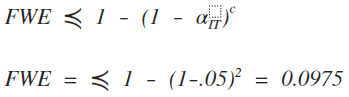
\includegraphics{/Users/cwong79/Dropbox/Public/CUNY/DATA 605/final-a.png}
\caption{}
\end{figure}

The FWE formula states that there is a 9.75\% probability there is an
error but I would not be worried as it is only applicable to larger
series of tests.

\subsection{5 points. Linear Algebra and Correlation. Invert your
correlation matrix from above. (This is known as the precision matrix
and contains variance inflation factors on the diagonal.) Multiply the
correlation matrix by the precision matrix, and then multiply the
precision matrix by the correlation matrix. Conduct LU decomposition on
the
matrix.}\label{points.-linear-algebra-and-correlation.-invert-your-correlation-matrix-from-above.-this-is-known-as-the-precision-matrix-and-contains-variance-inflation-factors-on-the-diagonal.-multiply-the-correlation-matrix-by-the-precision-matrix-and-then-multiply-the-precision-matrix-by-the-correlation-matrix.-conduct-lu-decomposition-on-the-matrix.}

\begin{Shaded}
\begin{Highlighting}[]
\NormalTok{t2 <-}\StringTok{ }\KeywordTok{cor}\NormalTok{(trainsub1)}

\NormalTok{precision_mat <-}\StringTok{ }\KeywordTok{solve}\NormalTok{(t2)}

\NormalTok{cmpm <-}\StringTok{ }\NormalTok{t2 }\OperatorTok\StringTok{ }\NormalTok{precision_mat}
\NormalTok{cmpm}
\end{Highlighting}
\end{Shaded}

\begin{verbatim}
##                 LotArea     GrLivArea    SalePrice
## LotArea    1.000000e+00  0.000000e+00 0.000000e+00
## GrLivArea  1.387779e-17  1.000000e+00 2.220446e-16
## SalePrice -2.775558e-17 -2.220446e-16 1.000000e+00
\end{verbatim}

\begin{Shaded}
\begin{Highlighting}[]
\NormalTok{pmcm <-}\StringTok{ }\NormalTok{precision_mat }\OperatorTok\StringTok{ }\NormalTok{t2}
\NormalTok{pmcm}
\end{Highlighting}
\end{Shaded}

\begin{verbatim}
##                 LotArea   GrLivArea    SalePrice
## LotArea    1.000000e+00 1.94289e-16 1.387779e-16
## GrLivArea -1.110223e-16 1.00000e+00 0.000000e+00
## SalePrice -1.110223e-16 0.00000e+00 1.000000e+00
\end{verbatim}

\begin{Shaded}
\begin{Highlighting}[]
\KeywordTok{lu}\NormalTok{(t2)}
\end{Highlighting}
\end{Shaded}

\begin{verbatim}
## $L
##             LotArea GrLivArea SalePrice
## LotArea   1.0000000 0.0000000         0
## GrLivArea 0.2631162 1.0000000         0
## SalePrice 0.2638434 0.6867466         1
## 
## $U
##           LotArea GrLivArea SalePrice
## LotArea         1 0.2631162 0.2638434
## GrLivArea       0 0.9307699 0.6392030
## SalePrice       0 0.0000000 0.4914162
\end{verbatim}

\subsection{\texorpdfstring{5 points. Calculus-Based Probability \&
Statistics. Many times, it makes sense to fit a closed form distribution
to data. Select a variable in the Kaggle.com training dataset that is
skewed to the right, shift it so that the minimum value is absolutely
above zero if necessary. Then load the MASS package and run fitdistr to
fit an exponential probability density function. (See
\url{https://stat.ethz.ch/R-manual/R-devel/library/MASS/html/fitdistr.html}
). Find the optimal value of  for this distribution, and then take 1000
samples from this exponential distribution using this value (e.g.,
rexp(1000, )). Plot a histogram and compare it with a histogram of your
original variable. Using the exponential pdf, find the 5th and 95th
percentiles using the cumulative distribution function (CDF). Also
generate a 95\% confidence interval from the empirical data, assuming
normality. Finally, provide the empirical 5th percentile and 95th
percentile of the data.
Discuss.}{5 points. Calculus-Based Probability \& Statistics. Many times, it makes sense to fit a closed form distribution to data. Select a variable in the Kaggle.com training dataset that is skewed to the right, shift it so that the minimum value is absolutely above zero if necessary. Then load the MASS package and run fitdistr to fit an exponential probability density function. (See https://stat.ethz.ch/R-manual/R-devel/library/MASS/html/fitdistr.html ). Find the optimal value of  for this distribution, and then take 1000 samples from this exponential distribution using this value (e.g., rexp(1000, )). Plot a histogram and compare it with a histogram of your original variable. Using the exponential pdf, find the 5th and 95th percentiles using the cumulative distribution function (CDF). Also generate a 95\% confidence interval from the empirical data, assuming normality. Finally, provide the empirical 5th percentile and 95th percentile of the data. Discuss.}}\label{points.-calculus-based-probability-statistics.-many-times-it-makes-sense-to-fit-a-closed-form-distribution-to-data.-select-a-variable-in-the-kaggle.com-training-dataset-that-is-skewed-to-the-right-shift-it-so-that-the-minimum-value-is-absolutely-above-zero-if-necessary.-then-load-the-mass-package-and-run-fitdistr-to-fit-an-exponential-probability-density-function.-see-httpsstat.ethz.chr-manualr-devellibrarymasshtmlfitdistr.html-.-find-the-optimal-value-of-for-this-distribution-and-then-take-1000-samples-from-this-exponential-distribution-using-this-value-e.g.-rexp1000-.-plot-a-histogram-and-compare-it-with-a-histogram-of-your-original-variable.-using-the-exponential-pdf-find-the-5th-and-95th-percentiles-using-the-cumulative-distribution-function-cdf.-also-generate-a-95-confidence-interval-from-the-empirical-data-assuming-normality.-finally-provide-the-empirical-5th-percentile-and-95th-percentile-of-the-data.-discuss.}

\begin{Shaded}
\begin{Highlighting}[]
\KeywordTok{hist}\NormalTok{(trainsub1}\OperatorTok{$}\NormalTok{SalePrice,}\DataTypeTok{main=}\StringTok{"Distribution of Price"}\NormalTok{,}\DataTypeTok{xlab=}\StringTok{"Sale Price"}\NormalTok{)}
\end{Highlighting}
\end{Shaded}

\includegraphics{Cwong_Final_Project_files/figure-latex/unnamed-chunk-16-1.pdf}

\begin{Shaded}
\begin{Highlighting}[]
\NormalTok{(fd <-}\StringTok{ }\KeywordTok{fitdistr}\NormalTok{(trainsub1}\OperatorTok{$}\NormalTok{SalePrice, }\StringTok{"exponential"}\NormalTok{))}
\end{Highlighting}
\end{Shaded}

\begin{verbatim}
##        rate    
##   5.527268e-06 
##  (1.446552e-07)
\end{verbatim}

\begin{Shaded}
\begin{Highlighting}[]
\NormalTok{generated <-}\StringTok{ }\KeywordTok{rexp}\NormalTok{(}\DecValTok{1000}\NormalTok{, }\DataTypeTok{rate =}\NormalTok{ fd}\OperatorTok{$}\NormalTok{estimate)}

\KeywordTok{hist}\NormalTok{(trainsub1}\OperatorTok{$}\NormalTok{SalePrice, }\DataTypeTok{breaks=}\DecValTok{30}\NormalTok{, }\DataTypeTok{prob=}\OtherTok{TRUE}\NormalTok{, }\DataTypeTok{xlab=}\StringTok{"Sale Price"}\NormalTok{, }\DataTypeTok{main=}\StringTok{"Real Price Distribution"}\NormalTok{)}
\end{Highlighting}
\end{Shaded}

\includegraphics{Cwong_Final_Project_files/figure-latex/unnamed-chunk-16-2.pdf}

\begin{Shaded}
\begin{Highlighting}[]
\KeywordTok{hist}\NormalTok{(generated, }\DataTypeTok{breaks=}\DecValTok{30}\NormalTok{, }\DataTypeTok{prob=}\OtherTok{TRUE}\NormalTok{, }\DataTypeTok{xlab=}\StringTok{"Generated Data"}\NormalTok{, }\DataTypeTok{main=}\StringTok{"Generated Price Distribution"}\NormalTok{)}
\end{Highlighting}
\end{Shaded}

\includegraphics{Cwong_Final_Project_files/figure-latex/unnamed-chunk-16-3.pdf}

\subsubsection{Find the 5th and 95th percentiles using the cumulative
distribution function
(CDF)}\label{find-the-5th-and-95th-percentiles-using-the-cumulative-distribution-function-cdf}

\begin{Shaded}
\begin{Highlighting}[]
\NormalTok{Fn <-}\StringTok{ }\KeywordTok{ecdf}\NormalTok{(generated)}
\NormalTok{generated[}\KeywordTok{Fn}\NormalTok{(generated)}\OperatorTok{==}\FloatTok{0.05}\NormalTok{]}
\end{Highlighting}
\end{Shaded}

\begin{verbatim}
## [1] 10913.91
\end{verbatim}

\begin{Shaded}
\begin{Highlighting}[]
\NormalTok{generated[}\KeywordTok{Fn}\NormalTok{(generated)}\OperatorTok{==}\FloatTok{0.95}\NormalTok{]}
\end{Highlighting}
\end{Shaded}

\begin{verbatim}
## [1] 506295.1
\end{verbatim}

\subsubsection{Generate a 95\% confidence interval from the empirical
data, assuming
normality.}\label{generate-a-95-confidence-interval-from-the-empirical-data-assuming-normality.}

\begin{Shaded}
\begin{Highlighting}[]
\KeywordTok{ci}\NormalTok{(trainsub1}\OperatorTok{$}\NormalTok{SalePrice, }\FloatTok{0.95}\NormalTok{)}
\end{Highlighting}
\end{Shaded}

\begin{verbatim}
## Warning in ci.numeric(trainsub1$SalePrice, 0.95): No class or unkown class.
## Using default calcuation.
\end{verbatim}

\begin{verbatim}
##   Estimate   CI lower   CI upper Std. Error 
## 180921.196 176842.841 184999.551   2079.105
\end{verbatim}

\subsubsection{Provide the empirical 5th percentile and 95th percentile
of the
data.}\label{provide-the-empirical-5th-percentile-and-95th-percentile-of-the-data.}

\begin{Shaded}
\begin{Highlighting}[]
\KeywordTok{quantile}\NormalTok{(trainsub1}\OperatorTok{$}\NormalTok{SalePrice, .}\DecValTok{05}\NormalTok{)}
\end{Highlighting}
\end{Shaded}

\begin{verbatim}
##    5% 
## 88000
\end{verbatim}

\begin{Shaded}
\begin{Highlighting}[]
\KeywordTok{quantile}\NormalTok{(trainsub1}\OperatorTok{$}\NormalTok{SalePrice, .}\DecValTok{95}\NormalTok{)}
\end{Highlighting}
\end{Shaded}

\begin{verbatim}
##    95% 
## 326100
\end{verbatim}

\subsection{10 points. Modeling. Build some type of multiple regression
model and submit your model to the competition board. Provide your
complete model summary and results with analysis. Report your Kaggle.com
user name and
score.}\label{points.-modeling.-build-some-type-of-multiple-regression-model-and-submit-your-model-to-the-competition-board.-provide-your-complete-model-summary-and-results-with-analysis.-report-your-kaggle.com-user-name-and-score.}

Lets look at numerical variables and see how they stack up against sale
price. I wanted to pick variables with higher than .6 correlation and
run it through a regression model to see how R values read.

\begin{Shaded}
\begin{Highlighting}[]
\NormalTok{numericVars <-}\StringTok{ }\KeywordTok{which}\NormalTok{(}\KeywordTok{sapply}\NormalTok{(train.df, is.numeric)) }
\NormalTok{numericVarNames <-}\StringTok{ }\KeywordTok{names}\NormalTok{(numericVars) }

\NormalTok{all_numVar <-}\StringTok{ }\NormalTok{train.df[, numericVars] }
\NormalTok{all_numVar <-}\StringTok{ }\NormalTok{all_numVar[ }\OperatorTok{-}\KeywordTok{c}\NormalTok{(}\DecValTok{1}\NormalTok{) ]}
\NormalTok{cor_numVar <-}\StringTok{ }\KeywordTok{cor}\NormalTok{(all_numVar, }\DataTypeTok{use=}\StringTok{"pairwise.complete.obs"}\NormalTok{) }

\NormalTok{cor_sorted <-}\StringTok{ }\KeywordTok{as.matrix}\NormalTok{(}\KeywordTok{sort}\NormalTok{(cor_numVar[,}\StringTok{'SalePrice'}\NormalTok{], }\DataTypeTok{decreasing =} \OtherTok{TRUE}\NormalTok{))}
 
\NormalTok{CorHigh <-}\StringTok{ }\KeywordTok{names}\NormalTok{(}\KeywordTok{which}\NormalTok{(}\KeywordTok{apply}\NormalTok{(cor_sorted, }\DecValTok{1}\NormalTok{, }\ControlFlowTok{function}\NormalTok{(x) }\KeywordTok{abs}\NormalTok{(x)}\OperatorTok{>}\FloatTok{0.6}\NormalTok{)))}
\NormalTok{cor_numVar <-}\StringTok{ }\NormalTok{cor_numVar[CorHigh, CorHigh]}
\KeywordTok{corrplot.mixed}\NormalTok{(cor_numVar, }\DataTypeTok{tl.col=}\StringTok{"black"}\NormalTok{, }\DataTypeTok{tl.pos =} \StringTok{"lt"}\NormalTok{)}
\end{Highlighting}
\end{Shaded}

\includegraphics{Cwong_Final_Project_files/figure-latex/unnamed-chunk-20-1.pdf}

For building model I've removed the variables with less than 0.6
correlation to sale price. After that I've fitted a multiple regression
model. A step wise regression to select best set of predictor variables.
My model's R square value is at 0.7609. Since the p-value is less than
0.05 at a 5\% significant level, we can surmice that the model is valid.

\begin{Shaded}
\begin{Highlighting}[]
\NormalTok{model <-}\StringTok{ }\KeywordTok{lm}\NormalTok{(SalePrice }\OperatorTok{~}\StringTok{ }\NormalTok{., }\DataTypeTok{data =}\NormalTok{ all_numVar[CorHigh])}
\KeywordTok{summary}\NormalTok{(model)}
\end{Highlighting}
\end{Shaded}

\begin{verbatim}
## 
## Call:
## lm(formula = SalePrice ~ ., data = all_numVar[CorHigh])
## 
## Residuals:
##     Min      1Q  Median      3Q     Max 
## -473373  -19732   -1080   16922  288035 
## 
## Coefficients:
##               Estimate Std. Error t value Pr(>|t|)    
## (Intercept) -1.027e+05  4.904e+03 -20.932  < 2e-16 ***
## OverallQual  2.400e+04  1.083e+03  22.150  < 2e-16 ***
## GrLivArea    4.312e+01  2.679e+00  16.095  < 2e-16 ***
## GarageCars   1.452e+04  3.019e+03   4.809 1.68e-06 ***
## GarageArea   1.566e+01  1.047e+01   1.495   0.1350    
## TotalBsmtSF  2.439e+01  4.318e+00   5.649 1.94e-08 ***
## X1stFlrSF    1.119e+01  5.032e+00   2.223   0.0264 *  
## ---
## Signif. codes:  0 '***' 0.001 '**' 0.01 '*' 0.05 '.' 0.1 ' ' 1
## 
## Residual standard error: 38840 on 1453 degrees of freedom
## Multiple R-squared:  0.7619, Adjusted R-squared:  0.7609 
## F-statistic:   775 on 6 and 1453 DF,  p-value: < 2.2e-16
\end{verbatim}


\end{document}
